% This is "sig-alternate.tex" V2.1 April 2013
% This file should be compiled with V2.5 of "sig-alternate.cls" May 2012
%
% This example file demonstrates the use of the 'sig-alternate.cls'
% V2.5 LaTeX2e document class file. It is for those submitting
% articles to ACM Conference Proceedings WHO DO NOT WISH TO
% STRICTLY ADHERE TO THE SIGS (PUBS-BOARD-ENDORSED) STYLE.
% The 'sig-alternate.cls' file will produce a similar-looking,
% albeit, 'tighter' paper resulting in, invariably, fewer pages.
%
% ----------------------------------------------------------------------------------------------------------------
% This .tex file (and associated .cls V2.5) produces:
%       1) The Permission Statement
%       2) The Conference (location) Info information
%       3) The Copyright Line with ACM data
%       4) NO page numbers
%
% as against the acm_proc_article-sp.cls file which
% DOES NOT produce 1) thru' 3) above.
%
% Using 'sig-alternate.cls' you have control, however, from within
% the source .tex file, over both the CopyrightYear
% (defaulted to 200X) and the ACM Copyright Data
% (defaulted to X-XXXXX-XX-X/XX/XX).
% e.g.
% \CopyrightYear{2007} will cause 2007 to appear in the copyright line.
% \crdata{0-12345-67-8/90/12} will cause 0-12345-67-8/90/12 to appear in the copyright line.
%
% ---------------------------------------------------------------------------------------------------------------
% This .tex source is an example which *does* use
% the .bib file (from which the .bbl file % is produced).
% REMEMBER HOWEVER: After having produced the .bbl file,
% and prior to final submission, you *NEED* to 'insert'
% your .bbl file into your source .tex file so as to provide
% ONE 'self-contained' source file.
%
% ================= IF YOU HAVE QUESTIONS =======================
% Questions regarding the SIGS styles, SIGS policies and
% procedures, Conferences etc. should be sent to
% Adrienne Griscti (griscti@acm.org)
%
% Technical questions _only_ to
% Gerald Murray (murray@hq.acm.org)
% ===============================================================
%
% For tracking purposes - this is V2.0 - May 2012

\documentclass{sig-alternate-05-2015}
\usepackage[utf8]{inputenc}
\usepackage{pdflscape}

\begin{document}

% Copyright
%\setcopyright{acmcopyright}
%\setcopyright{acmlicensed}
%\setcopyright{rightsretained}
%\setcopyright{usgov}
%\setcopyright{usgovmixed}
%\setcopyright{cagov}
%\setcopyright{cagovmixed}


% DOI
%\doi{10.475/123_4}

% ISBN
%\isbn{123-4567-24-567/08/06}

%Conference
\conferenceinfo{AsianPLoP 2016}{February 24-26, Taiwan.}

%\acmPrice{\$15.00}

%
% --- Author Metadata here ---
%\conferenceinfo{WOODSTOCK}{'97 El Paso, Texas USA}
%\CopyrightYear{2007} % Allows default copyright year (20XX) to be over-ridden - IF NEED BE.
%\crdata{0-12345-67-8/90/01}  % Allows default copyright data (0-89791-88-6/97/05) to be over-ridden - IF NEED BE.
% --- End of Author Metadata ---

\title{A Misuse Pattern for Web Browsers: Interception of traffic}
%\subtitle{[Extended Abstract]
%\titlenote{A full version of this paper is available as
%\textit{Author's Guide to Preparing ACM SIG Proceedings Using
%\LaTeX$2_\epsilon$\ and BibTeX} at


\numberofauthors{3} %  in this sample file, there are a *total*
% of EIGHT authors. SIX appear on the 'first-page' (for formatting
% reasons) and the remaining two appear in the \additionalauthors section.
%

\author{
\alignauthor
Paulina Silva\\
  \affaddr{Departamento de Informática}\\
  \affaddr{Universidad Técnica Federico Santa María}\\
  \affaddr{Valparaíso, Chile}\\
  \email{pasilva@alumnos.inf.utfsm.cl}
% 2nd. author
\alignauthor
Raúl Monge\\
  \affaddr{Departamento de Informática}\\
  \affaddr{Universidad Técnica Federico Santa María}\\
  \affaddr{Valparaíso, Chile}\\
  \email{rmonge@inf.utfsm.cl}
% 3rd. author
\alignauthor 
Eduardo B. Fernandez\\
  \affaddr{Department of Computer \(\&\) Electrical Engineering and Computer Science}\\
  \affaddr{Florida Atlantic University}\\
  \affaddr{Boca Raton, Fl, USA}\\
  \email{fernande@fau.edu}
}

\maketitle
\begin{abstract}
Currently, most software development is focused in creating systems connected to the Internet, which allows to add functionality within a system and facilities to their \textit{Stakeholders}. This leads to depend on a \textit{web client}, such as \textit{Web Browser}, which allows access to services, data or operations that the system delivers. However, the Internet influences the attack surface of the system, and unfortunately many stakeholders and developers are not aware of the risks to which they are exposed. The lack of security education among software developers and the scarce and scattered documentation for browsers (and standardization) could become a big problem in large architectural developments that depend on browsers to perform their services. We are studying some security attacks in the web browser by describing them in the form of misuse patterns. A misuse pattern describes how an information misuse is performed from the point of view of the attacker. It defines the environment where the attack is performed, how the attack is performed, countermeasures to stop it, and how to find forensic information to trace the attack once it happens. We are building a catalog of misuse patterns and we present here one we call Interception of traffic in the Web Browser. A catalog of misuse patterns will help designers to evaluate their designs for possible threats.
\end{abstract}


%
% The code below should be generated by the tool at
% http://dl.acm.org/ccs.cfm
% Please copy and paste the code instead of the example below. 
%
\begin{CCSXML}
<ccs2012>
 <concept>
  <concept_id>10010520.10010553.10010562</concept_id>
  <concept_desc>Computer systems organization~Embedded systems</concept_desc>
  <concept_significance>500</concept_significance>
 </concept>
 <concept>
  <concept_id>10010520.10010575.10010755</concept_id>
  <concept_desc>Computer systems organization~Redundancy</concept_desc>
  <concept_significance>300</concept_significance>
 </concept>
 <concept>
  <concept_id>10010520.10010553.10010554</concept_id>
  <concept_desc>Computer systems organization~Robotics</concept_desc>
  <concept_significance>100</concept_significance>
 </concept>
 <concept>
  <concept_id>10003033.10003083.10003095</concept_id>
  <concept_desc>Networks~Network reliability</concept_desc>
  <concept_significance>100</concept_significance>
 </concept>
</ccs2012>  
\end{CCSXML}

\ccsdesc[500]{Computer systems organization~Embedded systems}
\ccsdesc[300]{Computer systems organization~Redundancy}
\ccsdesc{Computer systems organization~Robotics}
\ccsdesc[100]{Networks~Network reliability}




\keywords{Browser, Web Client, Misuse Pattern, Security, Man-in-the-Browser}

\section{Introduction}
%hablar sobre ataques de ingeniería social
The current scenario of attacks in the browser has changed considerably, if compared to those browsers in the 90s. Every day browsers are more robust and difficult to exploit; therefore, the same attack types, such as drive-by downloads or code-based execution that could subvert a system, are less common every time. A new form of attack has emerged and is fairly easy to achieve, because it is based on deceiving the user to perform what the attacker wants. Once the user is tricked, the attacker can achieve total control over the browser or the host, without having to crack the system \cite{Rajab2013,Labs2013} that hosts the browser. The development of critical systems that interact daily with different users on the network should focus on these attacks because they threaten the confidentiality, integrity and availability of the user's data (personal) as well as the Stakeholders involved.

The new type of attacks described above are called ``social engineering attacks", in \cite{socEngineeering} they are defined as: The act of manipulating someone to perform actions that are not part of the best interests of the victim (person, organization, stakeholder, etc). An attack of this kind can take many forms, there is the possibility of a physical or digital encounter with the victim. Based on social engineering, this attack is one that takes advantage of human behavior and trust of the victim. In the context of web browser, the deceived user is the first and last line of defense against such attacks, the abuse of trust of the user may open the doors of the browser's host, causing damage to both the user and the external systems with which it interacts.

According to studies \cite{browSecPhish,Labs2013,rowSecSEMBlock}, the browser is the first line of defense against multiple Web threats. However, this is affected by the lack of education of users who use browsers and the constant evolution of threats \cite{browSecPhish}. This is why many browser manufacturers have created defense mechanisms such as those shown in \cite{Drake2011}, that act when the user requests a page, including black or white lists, reputation systems \cite{Rajab2013} with warning alerts, among others, so the user can at least avoid the page or choose to enter the malicious site anyway (but no granting access to the page without knowing of the threat).

In this work, a Misuse Pattern is presented as a first step in to the process of creating a catalog of misuses for the Web Browser. A catalog of misuse patterns will help designers to evaluate their designs for possible attacks. The audience to which our paper is focused are Browser developers, Web Application developers and even normal users. Being the first two the most important, since they are the responsible for the implementation and correct use of secure mechanisms while a user is browsing in the Internet. Secure communication is an important matter, but in this work the focus will be on the Browser and how to control the responses it receives.


\section{Misuse Pattern: Interception of traffic in the Web Browser}
\subsection*{Intent}
An attacker could modify or spy the traffic when the Browser User sends a request or receives the response from the Provider to the Browser Kernel; by doing so, the browser could interpret the information in a different way than if it had received the original traffic.

\subsection*{Context}
A web browser fetches resources (web pages, services, etc.) from a Provider to satisfy the access of a Browser User. The Provider is generally a Web App or Web server, that allows input and output of data to other applications, and usually they are built using HTML, Javascript and CCS. A Provider, depending on its type, can receive many requests for resources from various hosts. Depending on the type of request, they may or may not be accepted. For those accepted, the Provider generates a response to the Host, which may go back (or not) to the Browser Kernel that generated the request.

\subsection*{Problem}
An attacker tries to take advantage of any input the Browser User requests to affect the system. Users may be tricked by social engineering attacks, or lead into downloading and executing a binary in the browser to affect the Renderer that may have unprotected vulnerabilities. Therefore it is possible to give the attacker a chance to hide in the middle of the communication between the browser's processes, resulting in the interception of content that may affect the Renderer or the browser itself. Depending on the type of attacker, it is possible that it may even affect the host where the browser is.

The solution is affected by the following forces:
\begin{itemize}
  \item Misuse: Perform some destruction and/or other misuses (confidentiality and integrity).
  \item Stealthy/Untraceability: Try to hide its structure to make harder its detection and removal. Since it can compromises the host, it would be better if no one knows who is the responsible one. 
  \item Collateral damage: In addition to specific misuses, the attack may require difficult operations for stopping or disrupting browsers activities; web browser's basic knowledge is needed.
  \item Activation: This can be done by enticing offers which may tempt users to open email attachments or download procedures (social engineering).
\end{itemize}

The attack could take advantage of the following vulnerabilities:
\begin{itemize}
  \item The The Same Origin Policy (SOP) is defined by the \textbf{origin}, and is used to separate different resources by its domain, scheme and port (i.e: somedomain.com, http and 80). It is the minimun security mechanism a browser has while requesting cross-origin resources, and divides the different kind of contents so they can not interfere with each other. The SOP which every browser complies with, differs in every web browser manufacturer \cite{W3C-SOP,Reis2009, Jackson2008, Crowley2010, Paola2006}; for this reason, attackers take advantage to make malicious cross-origin requests.
  \item Attacker can take advantage of the flexibility the SOP has, because the \textbf{origin} is not enough as an isolation mechanism between the different resources \cite{Silic2010, Barth2009, Yason, Liu2012}. Different levels of isolation can give better results, but affecting the performance of the browser \cite{barth2008security,GoogleChromeIsolation}
  \item Anyone can create a software component like an extension or plugin for some type of web browser and pass it off as something harmless, consequently a user will not notice the threat and will install it. 
  %This could lead to a very known attack named Man-in-the-Browser \cite{Dougan2012,Utakrit2009,Liu2012,Barth2010}. Also, an installed malware (if the user with the required privileges was fooled to make the installation) could affect not only the traffic but also the logs of the systems, so it can erase its trace from the system.
  \item It is possible to affect the Browser Kernel, and in consequence the Host, without having to find a vulnerability in the system or browser. With social engineering methods it is possible to trick the user/victim into doing things that are not part of the best interests of the victim, because the Browser User is the weakest link in the system.
  \item The architecture to extend the browser functionality through extensions, plugins and other, depends on the manufacturer, and probably it has a large attack surface.
  \item No use or improper use of the Sandbox (No access control).
  \item Many browser manufacturers do not have robust defense mechanisms that allow an effective identification of malicious resources.
\end{itemize}

The attack can be facilitated by:
\begin{itemize}
  \item There are many tools for social engineering attacks, that tricks the Browser User into accepting the installation of extensions or malicious plugins more easily.
  \item Specially crafted scripts can be used to exploit the interpreter within the Renderer of the web browser (represented here as the Web Content Renderer). Often it is also possible to use the same scripting language elements to pass through certain security barriers provided by the SOP because the language is based on prototypes (ECMAscript). A prototype language is a style of object-oriented programming in which behaviour reuse or inheritance is performed via a process of cloning existing objects that serve as prototypes. Since the prototype is cloned for creating other objects, this could be uses to find new vulnerabilities within the Renderer of browsers.
  \item Encryption methods can do nothing against an attack that intercepts traffic before sending or after receiving a requested service/resource.
  \item There are browsers that still use a monolitic architecture (monoprocess). Meaning that the browser is using the users permission to access directly the host resources.
\end{itemize}
\subsection*{Solution}
An attacker can take advantage of the Browser User by letting a social engineering attack do its job, by surfing every website without distrust. If the Browser User is not careful, while surfing in the Internet, it could lead into downloading and installing malicious binaries in the system without notice. Also, a single phishing e-mail wishing for the user to click in a URL address could lead into installing a binaries, extensions or scripts in the Host. If a social engineering attack is successful the attacker can take its time, because whatever is installed in the Host, the attacker has installed it with the user's permission. Therefore every action done in the Host or Browser Kernel, will be identified by the Host as an action done by the Browser User, a user of the Host. 
If the attacker can obtain physical access to the Host running the Browser Kernel, he or she can install without the real user's consent an extension, script or binary in the Host, that could lead to a misuse. Also, is not a necessity for the attacker to install malicious payload/binaries in the Browser, she or he could use ``benign-but-buggy" extensions or scripts to surpass the Sandbox's secure mechanism and misuse the Host or Browser Kernel.


\subsection*{Structure}
In Figure \ref{fig:BIMisuse} the \textbf{Browser Kernel} is an entity that represents the main process of a Web Browser, which is constantly communicating with the host of the browser. A user who makes a \textbf{Request} to a Internet resources using a Web Browser, will be called \textbf{Browser User}. At the same time, a \textbf{Provider} is responsible for receiving external requests. According to the request, a \textbf{Provider} will send the \textbf{Service} (or resource) the \textbf{Browser User} needs in a \textbf{Response} message. Most Browsers use a central component to do operations that need to affect the Host of the Browser, a \textbf{Browser Kernel}. Figure \ref{fig:BIMisuse} shows the Class diagram for the Browser Infrastructure Pattern. For each new resource a \textbf{Browser Kernel} requests a created or reused \textbf{Web Content Renderer} instance; this will inherit the \textbf{Controlled Process} properties and its methods. A \textbf{Plugin} and an \textbf{Extension} are elements that extend the functionality of the browser; the extender being for the exclusive use of the browser while the plugin can be used in other systems, such as the Adobe Reader Plugin. A \textbf{Sandbox} is a Controlled Execution Domain \cite{fernandez2013security} created for a single \textbf{Controlled Process} instance. The \textbf{Sandbox} allows the process memory isolation and the access control of each communication between processes, such as an instance of a \textbf{Controlled Process} with the \textbf{Browser Kernel}; this applies to a \textbf{Web Content Renderer}, a \textbf{Plugin} and an \textbf{Extension} as well. To communicate with the \textbf{Browser Kernel}, a \textbf{Proxy} created within a \textbf{Controlled Process} forwards a \textbf{Local Request} to the \textbf{Reference Monitor} inside the \textbf{Browser Kernel}. For every message sent from a \textbf{Controlled Process}, the \textbf{Reference Monitor} will check the \textbf{Domain}'s \textbf{Right}s to permit the access. The access control which the Sandbox delivers to each \textbf{Controlled Process} allows the isolation between different \textbf{Domain}s. Depending on the manufacturer, a \textbf{Plugin} could not be Sandboxed. The \textbf{Attacker} class is a person using some unit that could undertake a risky action against the integrity and confidentiality of the browser, the user of it and Provider (Figure \ref{fig:BIMisuse}). The attacker is able to intercept the messages between the Browser Client and Controlled Process using a malicious Controlled Process, which could be instanced as a Plugin, Extension or a Web Content Renderer. A interception of the \textbf{Response} could also lead to the same misuse.

\begin{figure*}[h!t]
  \centering
  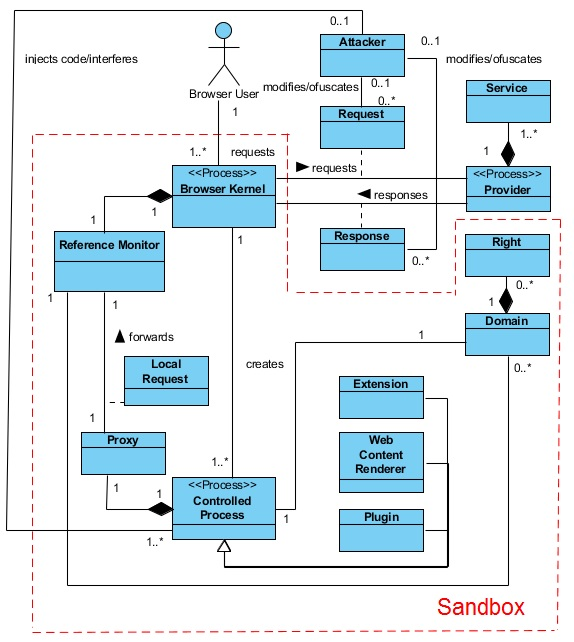
\includegraphics[scale=0.8]{figures/patronMisuse_v8.jpg}
  \caption{Class Diagram for the Misuse Pattern.}
  \label{fig:BIMisuse}
\end{figure*}

\subsection*{Dynamics}
In Figure \ref{fig:SeqMisuse} a series of required steps is shown, for one of the many misuses that can be made for the use case \textbf{Make Request}. The attacker is located between the Browser Kernel and the Controlled Processes, intercepting the original request or response and modifying the traffic to its taste; usually an attack based on this misuse is called Man-in-the-Browser (MITB) \cite{Liu2012, Barth2010, Utakrit2009, Dougan2012}. This could also happen when the Browser User has allowed the installation of plugins, extensions or external programs in the Host and Browser Kernel.

\begin{landscape}
\begin{figure*}[h!t]
  \centering
  \hspace*{-7cm}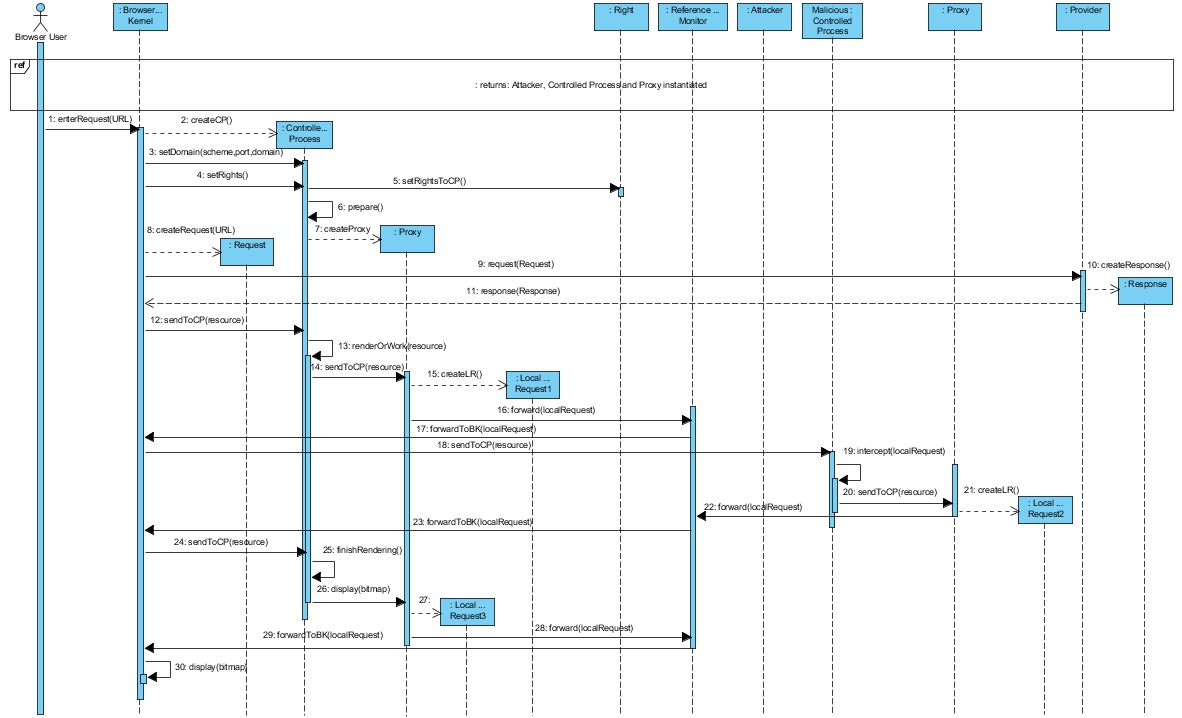
\includegraphics[scale=0.8]{figures/MakeRequestMisuse_v8.jpg}
  \caption{Sequence Diagram for the misuse: Interception of traffic in the Web Browser.}
  \label{fig:SeqMisuse}
\end{figure*}
\end{landscape}

  
  \subsubsection*{Summary} The attacker intercepts the traffic between the Browser Kernel and Controlled Processes. This action could lead to different kinds of misuses or new attacks depending on the attacker's intentions.
  \subsubsection*{Actor} Attacker
  \subsubsection*{Precondition} The Browser Kernel runs with the Browser User's permissions (a user in the Host), while interacts with limited privilege processes.

  \subsubsection*{Description}
      \begin{enumerate}
        \item An attacker uses a social engineering technique or vulnerability in the system, and creates an entity between the Browser Kernel and Controlled Process and their communication channel, normally a plugin, binary or extension. Also, an attacker could be using a ``benign-but-buggy" extension or script to the same purpose.
        \item A Browser User requires a browser to access a URL for some resource in a Provider, this is done by using a Browser Kernel already instanced in the Host. A Controlled Process and its Proxy are created or reused for rendering the resource needed. If the Controlled Process is new, the Domain and Rights of the Controlled Process are set.
        \item The Browser User requires the Host resources to obtain what is behind the URL. A Request is made from the Browser Kernel which creates a communication channel with the Provider, which in return sends a Response.
        \item The Browser Kernel receives the Response, and forwards it to the Controlled Process which the original Request came from.
        \item From here, the original or the ``may be" tapped Response could follow different ways. While rendering the resource, somewhere in the Response obtained the need of calling a plugin, an extension or a program for the rendering process will appear, and an action from the attacker to intercept the messages will occur. Also, a Browser Kernel could have been tapped to perform that action and send all the traffic to other Controlled Process; a malicious or to a ``benign-but-buggy". While sending the traffic, the Controlled Process needs to rely in its Proxy to send the data to the malicious plugin, extension or binary created through the Controlled Process. The traffic sent from the Controlled Process to the malicious one, has to make it through the Reference Monitor first, if the attacker wishes to be successful. The latter is done by sending a Local Request through the Proxy of the Controlled Process of origin, to the Reference Monitor in the Browser Kernel.
        \item Then, the Browser Kernel sends the traffic to the malicious or to a ``benign-but-buggy" Controlled Process and intercepts the traffic that is going to be used for rendering. Depending on the attacker's goals, the data can be spied or modified. Since the rendering process needs to finish, the intercepted traffic is returned through the Proxy in the malicious Controlled Process, to the Reference Monitor in the Browser Kernel, and then to the Controlled Process of origin to finish the rendering.
        \item It can happen the traffic goes between the malicious Controlled Process and the Browser Kernel several times before it can reach to the Controlled Process, in charge of the rendering process.
        \item Once the rendering process has finished, the bitmap is sent to the Browser Kernel (through the Proxy) and displayed in the Host. Also, the representation of the resource in the Web Content Renderer (DOM and data) could deviate from the original, thanks to the interception done by the attacker.

      \end{enumerate}
  \subsubsection*{Postconditions} The victim will be fully compromised and it probably will not be possible to detect the modification of a message, it is also possible that the log of the Host will be affected.

  \subsubsection*{Known Uses} The browser is a software that has different implementations, so the number of attack vectors are significant. Some of these are:
      \begin{itemize}
        \item Zeus \cite{zeus} is a Trojan horse malware that runs on Microsoft Windows and can be used to carry out many malicious and criminal tasks, it is often used to steal banking information by man-in-the-browser. First identified in July 2007 when it was used to steal information from the United States Department of Transportation.
        \item SpyEye \cite{spyeye1} is known as Zeus's successor, it is sophisticated botnet creation kit that has been implicated in a number of costly online banking thefts against businesses and consumers. One way people get infected is by visiting a website that has been tampered with by hackers. The site will contain a 1x1 pixel that pulls JavaScript from a different server and begins testing to see if the victim's computer has unpatched software.
        \item An extension based on the Google Chrome architecture or the Firefox WebExtension API could intercept the data before it reaches the Browser Kernel or Host \cite{Paola2006}. It could also be possible that a vulnerability in the extension or plugin is used by an attacker and takes advantage of its functionality to attack \cite{Liu2012,Barth2010}. Since the plugin, extension or process are elements the Host trust, it is possible that the attack is undetectable and the encryption methods do not serve as a mitigation measure.
        \item This type of attack can be used as base for more advanced attacks. For example, the browser could have \textit{cross-origin javascript capability leak} vulnerabilities, when different security models such as the one used by Javascript and the DOM interfere with each other. As a consequence, a \textit{cross-origin} request can perform even when the SOP was supposed to stop such attack \cite{Barth2009}. In 2009 a security bulletin regarding this type of vulnerability was issued \cite{javacapab}, where the getSVGDocument method was lacking an access check and allowed malicious a web site operator use the leaked capability to inject JavaScript into a target web site hosting an SVG document, bypassing the same-origin policy.
        %\item If neither an extension or plugin is used, a Troyan (a downloaded and executed binary) can be another way to get the Host and all the system compromised.
      \end{itemize}


\subsection*{Consequences}
The misuse has the following consequences for the attacker:
  \begin{itemize}
    \item Misuses: they may be different, we highlight vandalism, impersonate another person or monetary gain. While the attacker may be between the host and the traffic that is sent to the Provider, confidentiality and integrity of the data is completely lost even if the browser is communicating with a Provider through a secure channel. User privacy can no longer be assured.
    \item Stealthy/Untraceability: Since the attacker has managed to come between the system calls, that are made to the host, to send data to the Provider, the Host will not recognize or log the anomaly. Calls made to Host are perfectly legal and nothing out of the ordinary, so it will not be seen as something suspicious.
    \item Collateral damage: The attacker could perform actions that affect the integrity of the Host. The cost of fixing whatever the attack made on the host could have financial and organizational consequences.
  \item Activation: This can be done by enticing offers which may tempt users to open email attachments or download procedures (social engineering).
  \end{itemize}
  Possible sources of failure:
  \begin{itemize}
    \item If the Browser User is able to avoid or ignore the social engineering attack carried out at the beginning, this misuse can be avoided. 
    \item Also, this should consider that the user does not encounter pages with malicious content, which may affect other parts of a browser, but that would cause the same effect as the misuse presented here.
    \item If the browser manufacturers implement correctly the secure mechanism, the HTTP Only and Secure Cookie flags on the HTTP header could avoid the theft of session tokens, the use of cookies in scripts or the interception of data by a bystander.
  \end{itemize}

\subsection*{Countermeasures} 
  To prevent this kind of misuse we recommend taking the following preventive measures:
  \begin{itemize}
    \item Reputation services such as SmartScreen \cite{Colvin2010} from Internet Explorer and Download Application \cite{Rajab2013} from Google Chrome, can help identify pages, web content or resources that could contain malware when is installed as plugins, extensions or process in the Host of the User Browser.
    \item Providing education about the dangers while surfing the Internet and clarifying the users that they are the last line of defense against such attacks.
    \item Whitelist and Blacklist are installed in the browser as a preventive measure. They help avoid malicious pages or known malware while the user is browsing, they also are updated in a hourly-basis.
    \item Browsers like Google Chrome and Internet Explorer offer Sandboxing \cite{sandboxGC,Yason}. This defense mechanism limits the actions of the attacker which may affect the integrity of the system.
  \end{itemize}

\subsection*{Forensic Evidence}
  Where is it possible to find evidence? Depending on what is desired by the attacker, actions may differ. However the internal log of the browser could help in the audit of the system. This works until an attacker finds a vulnerability in the Sandbox or other component of the browser, in which case he can completely erase its tracks. Also, malware detection such as antivirus systems could help identifying tracks of misuses.

\subsection*{Related Patterns}
  \begin{itemize}
    \item The Browser Infrastructure pattern \cite{silva2015}.
    \item The Reified Reference Monitor \cite{fernandez2013security}, which describes how to enforce authorization rights when a subject requests access to a protected object or service and returns a decision (response). 
    \item The Sandbox is another name for the pattern Controlled Execution Domain \cite{fernandez2013security}.
    \item Blacklist and Whitelist patterns \cite{fernandez2013security}.
    \item The TLS pattern in \cite{fernandez2013security} complements our pattern, for adding security to communications between Client and Server.
  \end{itemize}


\section{Conclusions and future work}
%A Web browser appears to be a medium complexity software for users and developers without security experience, but unfortunately this piece of software allows a variaty of attack vectors, to the user using it as well the system with which interacts. Therefore it is important to understand its structure and how it interacts with internal or/and external Stakeholders.

%It is expected that in the future most \textit{Web Browser} will take the form of a Modular Architecture. Therefore, it is important that developers know the internal processes of \textit {browser} when developing a system that will interact with it. The Reference Architecture prepresented here, it is aimed at providing the basic knowledge of the components and interactions between \textit{Web Browser} and external Provider for resources; as well as the threats that exist within it.

%A part of our Reference Architecture has been built through the abstraction of found documentation, through the Browser Infrastructure pattern. We created our first architectural pattern for the infrastructure of \textit{Web Browser}; to help others to understand holistically the components, interactions and relationships of this system. Furthermore it has been possible to characterize the Stakeholders and one of the most important use case. From what we have known, this is the second Reference Architecture for the \textit{Browser} built.

%The proposed work allows a better understanding of this system called Web Browser by using our partially Reference Architecture, this is also helpful to understand existing threats. Furthermore, as it is not subject to specific implementations, it is possible to generalize certain results in other browsers.


We have presented a web browser attack as a misuse pattern that systematically describes how a misuse is performed. The aim is to understand and visualize the misuses of the browser that communicates with other systems, mainly to teach developers who have little (or none) security expertise. Through the list of threats shown in our previous work, it is possible to detect or infer misuse activities that may appear in one or more misuse cases.

With this misuse pattern we intent to initiate a catalog. This would help to condense the knowledge obtained using patterns so they can be used as guidelines to communicate relevant concepts, as well as evaluate the existent relationship between the browser and a developed system, to see what kind of interactions they have.

Future work to do is finishing the Reference Architecture for \textit{Web Browsers}. Other patterns related to Browser Infrastructure pattern will be obtained in order to complete the Reference Architecture, such as the Web Content Renderer and Browser Kernel pattern. 

We plan to build more Misuse Patterns for the Browser Infrastructure Pattern, to continue the study of the possible threats in the \textit{Browser}, as a way to educate Developers and Stakeholders. At the same time, these patterns will allow the construction of the Security Reference Architecture for the browser. In the same line, in addition to finding potential threats existing in the system, we need to find countermeasures or security defenses to prevent or foresee such threats through security patterns on the reference architecture built. An example of the type of work to be carried out can be seen in \cite{Fernandez2015}.

\bibliography{refTodas}  
\bibliographystyle{IEEEtran}


\end{document}
